\chapter{Results}
The three controllers are tested in the simulator, with several parameters logged at each frame for further evaluation, such as the Cartesian coordinates, \(cte\) and the steering angle. All three controllers are able to successfully drive around the track as shown in Figure \ref{coord}, however, there is a unique in how the neural network operates. Both rule-based controllers (PID \& MPC) depended on the track way points provided by the simulator, as well as the ground truth state of the vehicle to evaluate the error and cost function and accordingly output the relevant steering angle. On the other hand, the only input for the neural network is the image, which is a great advantage when considering implementing on a real vehicle, where such ground truth information is not available, but are rather the output of complicated computer vision and localization systems.
The Root Mean Squared error (RMSE) between the vehicle position and the center of the track is used as a Key Performance indicator (KPI) to compare the controllers.
\begin{figure}[htbp]
\centerline{
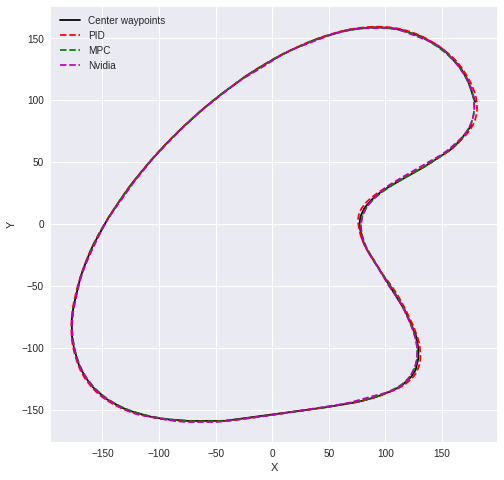
\includegraphics[width=0.8\linewidth]{plots/coord.png}}
\caption{The path taken by each controller compared to the track center way points}
\label{coord}
\end{figure}
\begin{figure}[htbp]
\centerline{
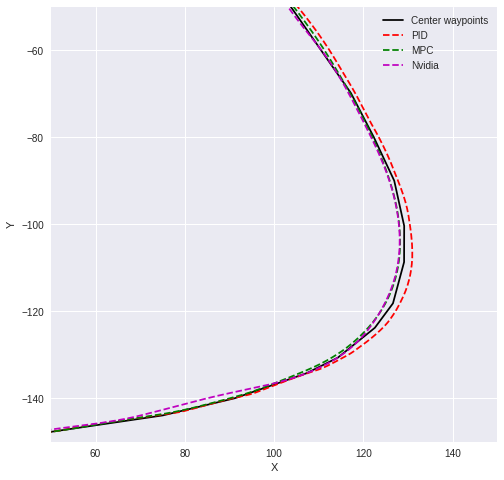
\includegraphics[width=0.8\linewidth]{plots/coord_1.png}}
\caption{First corner of the track}
\label{coord_1}
\end{figure}
\begin{figure}[htbp]
\centerline{
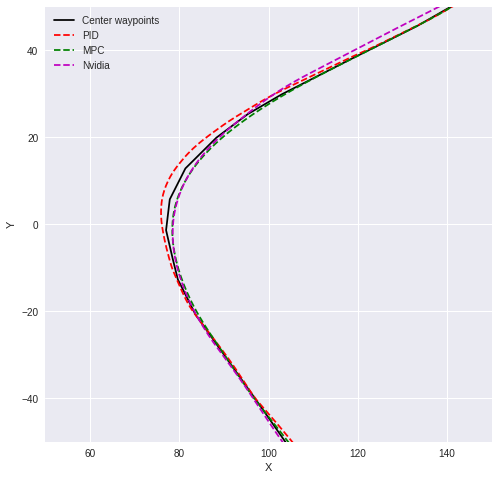
\includegraphics[width=0.8\linewidth]{plots/coord_2.png}}
\caption{Second corner of the track}
\label{coord_2}
\end{figure}

\begin{figure}[htbp]
\centerline{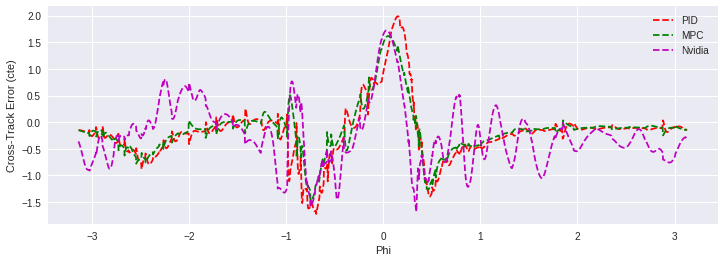
\includegraphics[width=\linewidth]{plots/cte.png}}
\caption{The logged \(cte\) values for each controller for a full lap}
\label{cte_plot}
\end{figure}
Table \ref{table:1} shows the RMSE value for each controller performing 1 complete lap around the track at \(30 mph\). These values are calculated based on the plotted values in Figure \ref{cte_plot}.
\begin{table}[ht]
\centering
\begin{tabular}{ |c|c|c| } 
\hline
Controller & RMSE \\
\hline
PID & 0.59477 \\ 
MPC & 0.47874 \\ 
CNN & 0.67840 \\ 
\hline 
\end{tabular}\\
\caption{RMSE evaluation of controllers}
\label{table:1}
\end{table}

The above table and plot indicate that the MPC is the top performing controller, followed by the PID, and finally the CNN when judged by the RMSE. However, the controller's behavior should also be considered when evaluating performance. Although PID performs better then the CNN from the RMSE perspective, it is obvious when observing the steering angle fluctuations that the CNN output is smoother than the PID. Since the CNN is trained to imitate the behavior of the MPC, the predicted steering angle smoothness of the CNN is very similar to that of the MPC. Unlike the MPC and the CNN, the PID output has several spikes in the steering command as shown in Figure \ref{steer}, which results in lateral jerk and a negative effect on ride comfort and quality when applied to passenger vehicles.\\
\begin{figure}[htbp]
\centerline{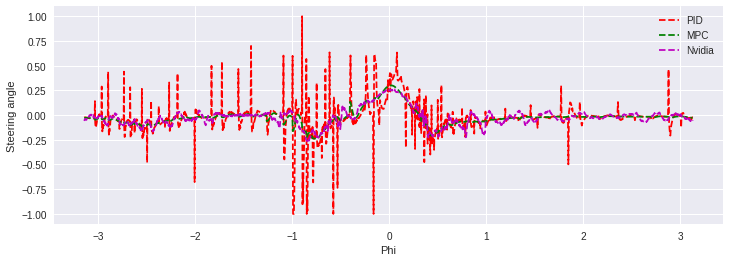
\includegraphics[width=\linewidth]{plots/steer.png}}
\caption{The logged predicted steering angles for each controller for a full lap}
\label{steer}
\end{figure}

To further understand the logic behind the functionality of the CNN and to explore its internal convolution filters, individual layer activations are extracted, merged, and visualized. The output is overlaid on the input image as shown in Figures \ref{activ} and \ref{activ_2}. It is observed that the CNN has learned to extract features that are representative of the road profile without being explicitly taught to do so.
\begin{figure}[htbp]
\centerline{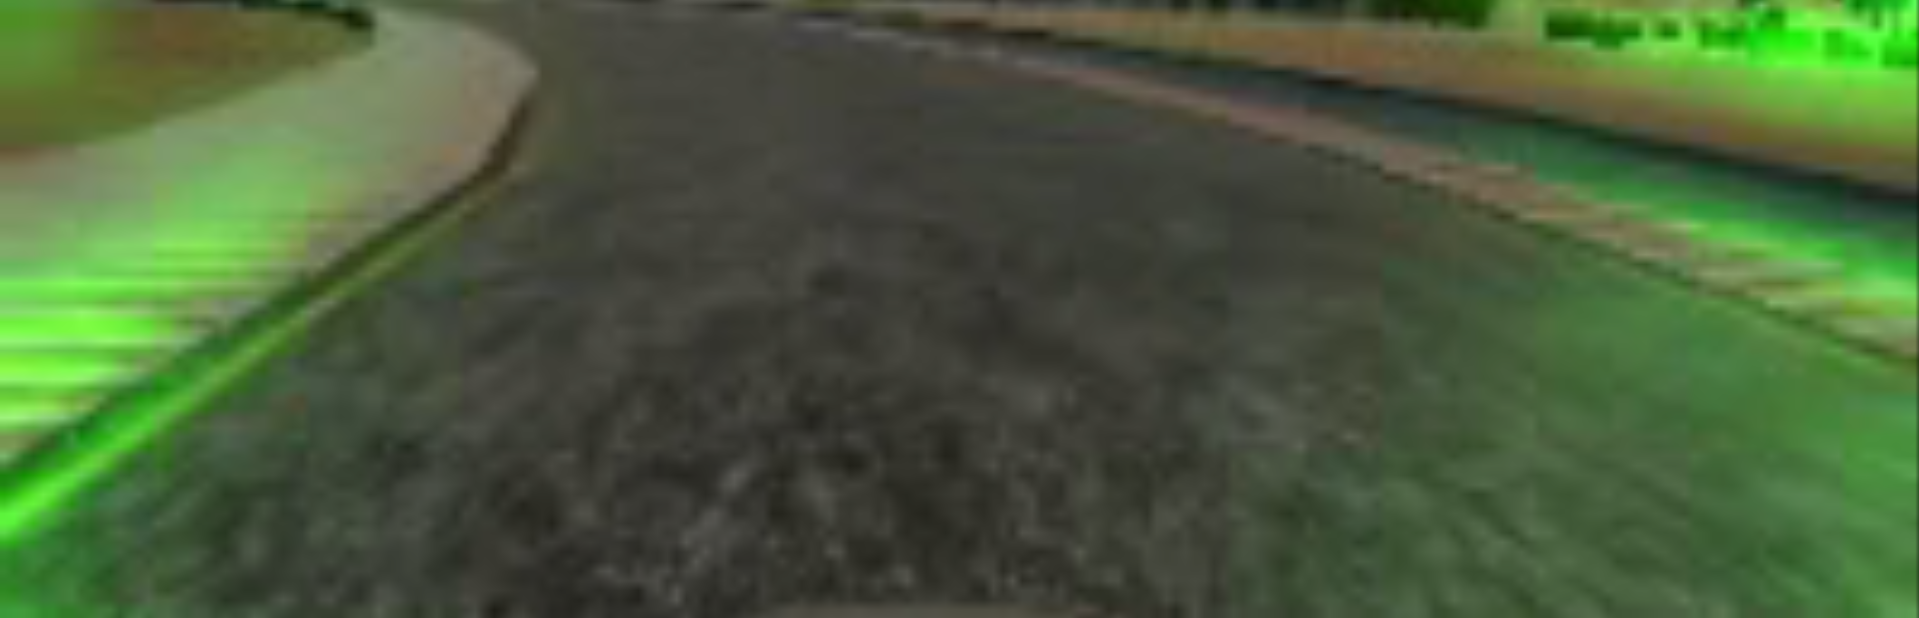
\includegraphics[width=\linewidth]{Figures/activations.PNG}}
\caption{Convolution layers activations overlaid on input image for a curved segment of the road}
\label{activ}
\end{figure}
\begin{figure}[htbp]
\centerline{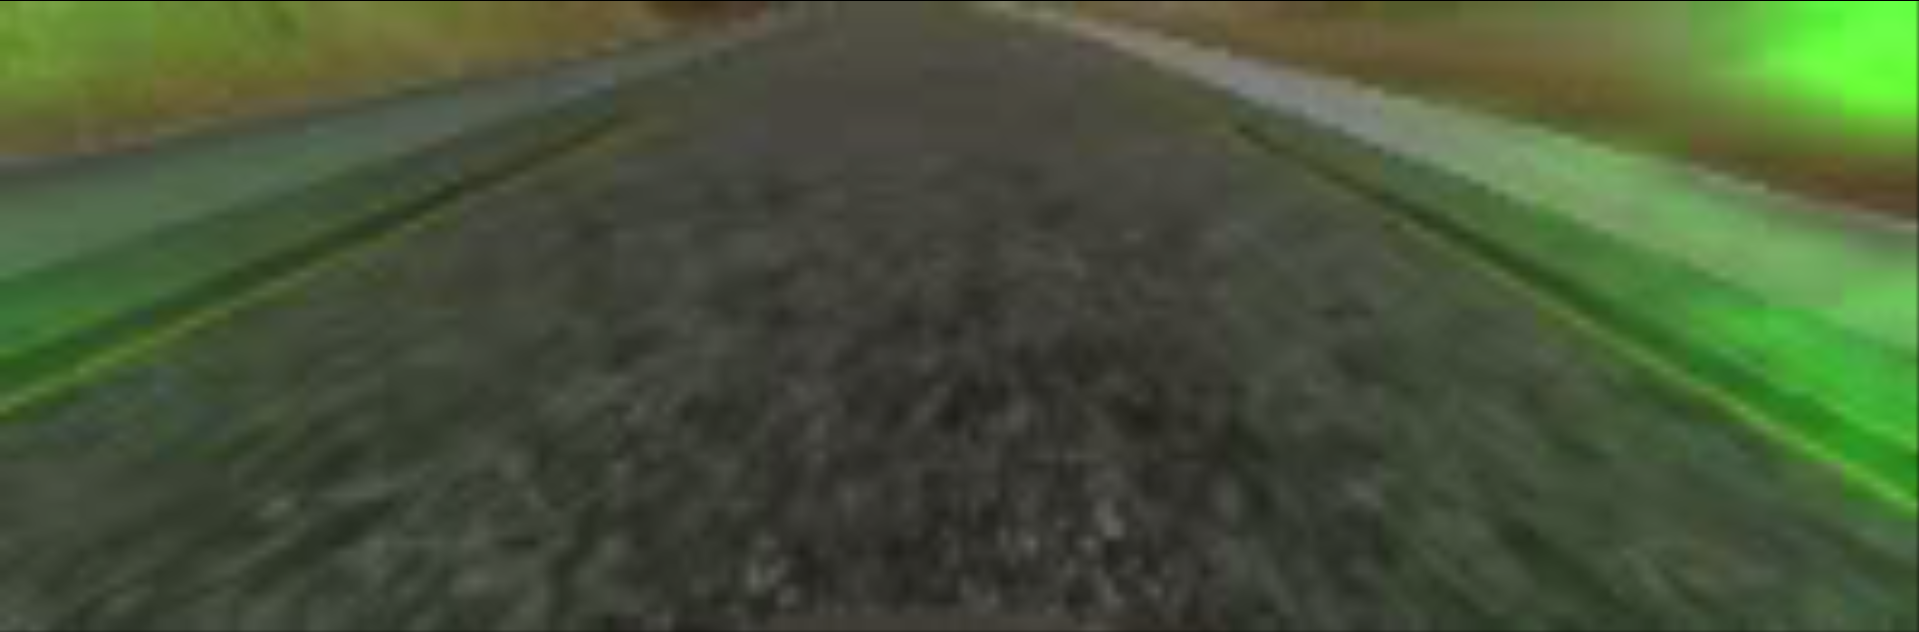
\includegraphics[width=\linewidth]{Figures/activations_2.PNG}}
\caption{Convolution layers activations overlaid on input image for a straight segment of the road}
\label{activ_2}
\end{figure}